\documentclass[11pt]{article}
\usepackage[margin=2cm]{geometry}
\usepackage{graphicx}
\usepackage{booktabs}
\usepackage{float}
\usepackage[hidelinks]{hyperref}

\title{DMMST --- Version 2 results:\\our loss variants compared with other models}
\author{Parsa}
\date{\today}

\begin{document}
\maketitle

\section{Setup}
We compare our model (a transformer with the survival head of the paper) trained with different
losses against eight published survival models. All models are run on the same five datasets
under the same protocol:
\begin{itemize}
  \item 10 random splits of each dataset (60\% train, 10\% validation, 30\% test);
        results are reported as mean (standard deviation) over the 10 splits;
  \item settings of every model chosen on the validation split only;
  \item every model scored by the same code.
\end{itemize}

\paragraph{Datasets.}
METABRIC and SUPPORT (real, one event: death);
EBMT (real, 4 events);
hsa synthetic and DeepHit synthetic (published synthetic data, 2 events).
SEER was planned as an additional large real dataset, but because of the updated SEER+
data-access policies we could not obtain access to it.

\paragraph{Our variants.}
\begin{center}
\begin{tabular}{ll}
\toprule
Name & Losses \\
\midrule
S1 & $L_{PCH}$ (survival likelihood) \\
S2 & $L_{PCH} + L_{rank}$ \\
S3 & $L_{PCH} + L_{mul}$ (multi-event data only) \\
S4 & $L_{PCH} + L_{rank} + L_{mul}$ (multi-event data only) \\
Full & survival head with all its losses + regression head ($L_{MAE}$ with best guess) \\
\bottomrule
\end{tabular}
\end{center}
$L_{mul}$ compares different events of the same patient, so S3 and S4 do not exist on
single-event data (``---'' in the tables).

\paragraph{Baselines.}
SurvTRACE (authors' code), DeepHit, RSF, PC-Hazard, DeepSurv, MENSA, Cox, DSM.

\paragraph{Scores.}
$C_{td}$: how well patients are ranked by risk (higher is better; 0.5 is random).
IBS: integrated Brier score, the accuracy of the predicted survival probabilities
(lower is better).

\section{Results}

\begin{table}[H]
\centering
\small
\caption{$C_{td}$, mean (sd) over 10 splits. Best per dataset in bold.}
\begin{tabular}{lccccc}
\toprule
Model & METABRIC & SUPPORT & EBMT & hsa synth. & DeepHit synth. \\
\midrule
Ours S1   & 0.667 (0.013) & 0.615 (0.011) & 0.529 (0.013) & 0.849 (0.049) & 0.743 (0.003) \\
Ours S2   & 0.670 (0.016) & 0.620 (0.007) & 0.535 (0.016) & \textbf{0.868} (0.010) & 0.743 (0.004) \\
Ours S3   & ---           & ---           & 0.530 (0.016) & 0.859 (0.015) & 0.742 (0.003) \\
Ours S4   & ---           & ---           & 0.537 (0.015) & 0.867 (0.009) & 0.742 (0.004) \\
Ours Full & 0.672 (0.021) & 0.619 (0.007) & 0.534 (0.017) & 0.852 (0.041) & 0.744 (0.004) \\
\midrule
SurvTRACE & \textbf{0.678} (0.013) & \textbf{0.638} (0.008) & 0.546 (0.009) & \textbf{0.868} (0.008) & 0.755 (0.007) \\
DeepHit   & 0.677 (0.012) & 0.610 (0.008) & 0.525 (0.011) & 0.865 (0.010) & 0.737 (0.006) \\
RSF       & 0.672 (0.014) & 0.636 (0.007) & \textbf{0.549} (0.009) & 0.849 (0.009) & 0.733 (0.005) \\
PC-Hazard & 0.668 (0.017) & 0.627 (0.008) & 0.548 (0.010) & 0.837 (0.008) & \textbf{0.762} (0.003) \\
DeepSurv  & 0.640 (0.030) & 0.593 (0.007) & 0.529 (0.014) & 0.842 (0.009) & \textbf{0.762} (0.002) \\
MENSA     & 0.654 (0.017) & 0.596 (0.021) & 0.501 (0.019) & 0.847 (0.014) & 0.570 (0.074) \\
Cox       & 0.631 (0.022) & 0.567 (0.006) & 0.531 (0.014) & 0.497 (0.013) & 0.591 (0.005) \\
DSM       & 0.620 (0.065) & 0.602 (0.037) & 0.512 (0.013) & 0.522 (0.031) & 0.653 (0.104) \\
\bottomrule
\end{tabular}
\end{table}

\begin{table}[H]
\centering
\small
\caption{Integrated Brier score (lower is better), mean (sd) over 10 splits. Best per dataset in bold.}
\begin{tabular}{lccccc}
\toprule
Model & METABRIC & SUPPORT & EBMT & hsa synth. & DeepHit synth. \\
\midrule
Ours S1   & 0.179 (0.012) & 0.200 (0.004) & 0.338 (0.165) & 0.075 (0.007) & 0.174 (0.005) \\
Ours S2   & 0.175 (0.006) & 0.199 (0.004) & 0.313 (0.153) & 0.075 (0.003) & 0.171 (0.005) \\
Ours S3   & ---           & ---           & 0.256 (0.082) & 0.074 (0.003) & 0.175 (0.005) \\
Ours S4   & ---           & ---           & 0.233 (0.043) & 0.075 (0.003) & 0.172 (0.006) \\
Ours Full & 0.177 (0.005) & 0.200 (0.003) & 0.299 (0.138) & 0.076 (0.005) & 0.172 (0.007) \\
\midrule
SurvTRACE & 0.201 (0.033) & \textbf{0.193} (0.004) & 0.242 (0.018) & \textbf{0.071} (0.003) & 0.169 (0.006) \\
DeepHit   & 0.198 (0.007) & 0.217 (0.004) & 0.388 (0.159) & 0.091 (0.002) & 0.254 (0.012) \\
RSF       & 0.176 (0.007) & \textbf{0.193} (0.003) & 0.224 (0.009) & 0.087 (0.002) & 0.185 (0.005) \\
PC-Hazard & \textbf{0.174} (0.006) & 0.194 (0.004) & 0.219 (0.010) & 0.078 (0.003) & 0.171 (0.005) \\
DeepSurv  & 0.176 (0.006) & 0.195 (0.004) & 0.220 (0.008) & 0.078 (0.003) & \textbf{0.167} (0.005) \\
MENSA     & 0.189 (0.012) & 0.212 (0.014) & 0.331 (0.023) & 0.079 (0.003) & 0.223 (0.014) \\
Cox       & 0.175 (0.006) & 0.198 (0.004) & \textbf{0.218} (0.009) & 0.105 (0.002) & 0.218 (0.006) \\
DSM       & 0.224 (0.067) & 0.205 (0.008) & 0.326 (0.024) & 0.369 (0.049) & 0.232 (0.078) \\
\bottomrule
\end{tabular}
\end{table}

\begin{figure}[H]
\centering
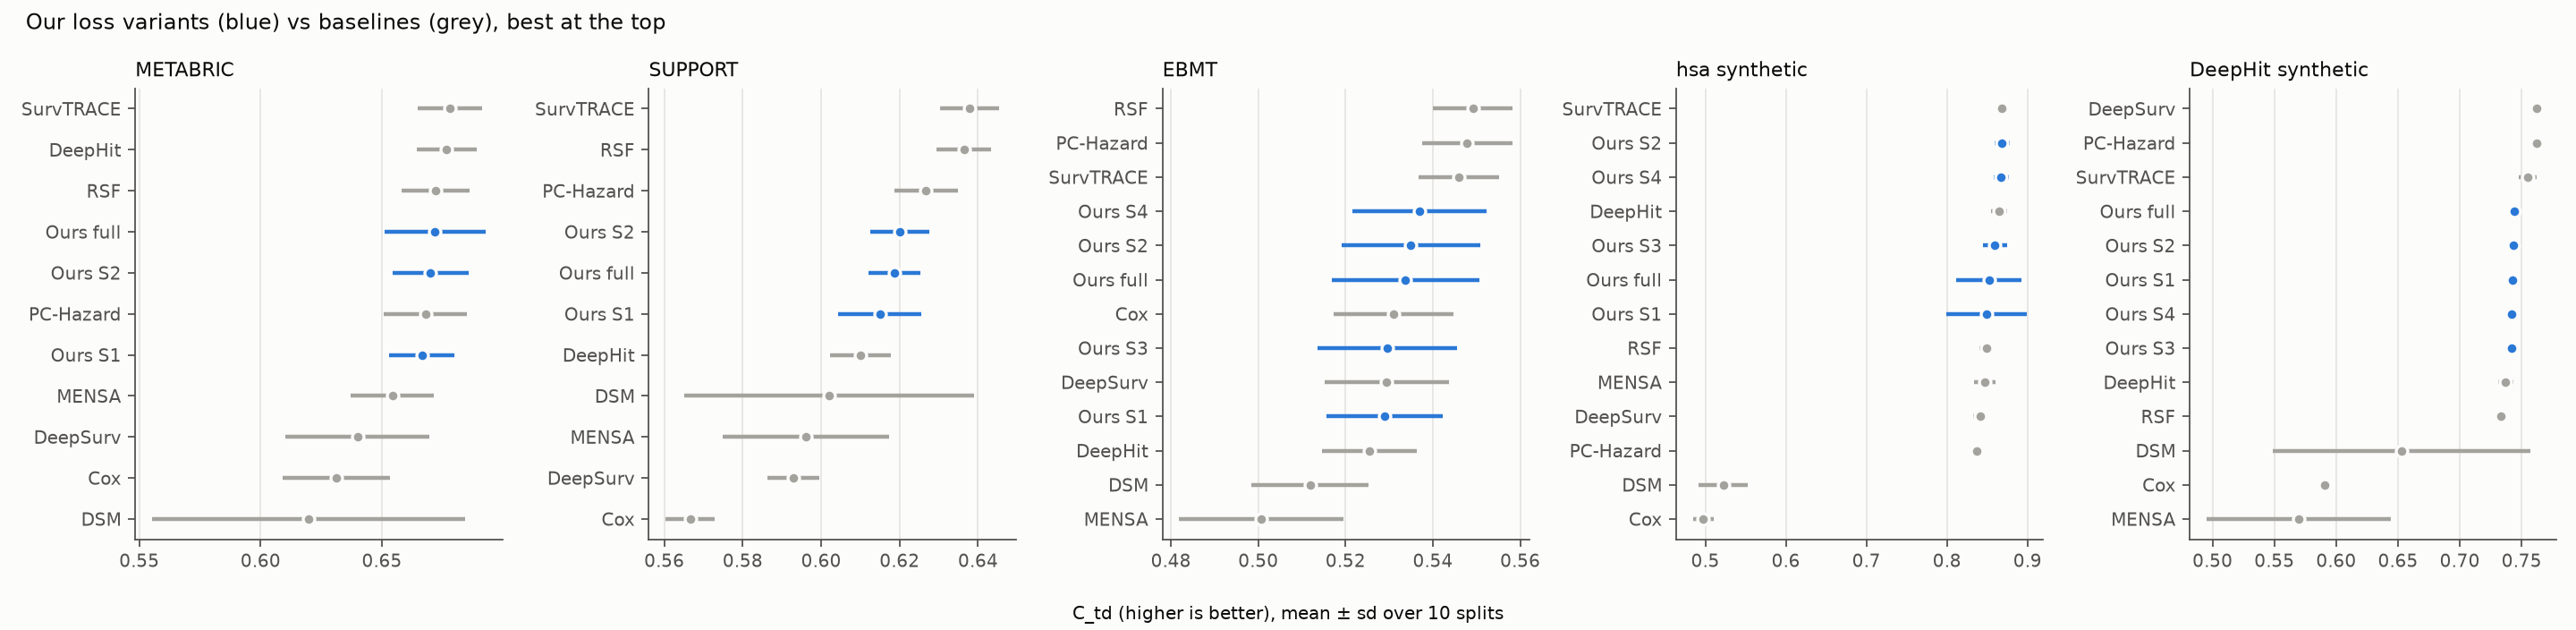
\includegraphics[width=\textwidth]{report_ctd.png}
\caption{$C_{td}$ of our variants (blue) and the baselines (grey), best at the top of each panel.}
\end{figure}

\begin{figure}[H]
\centering
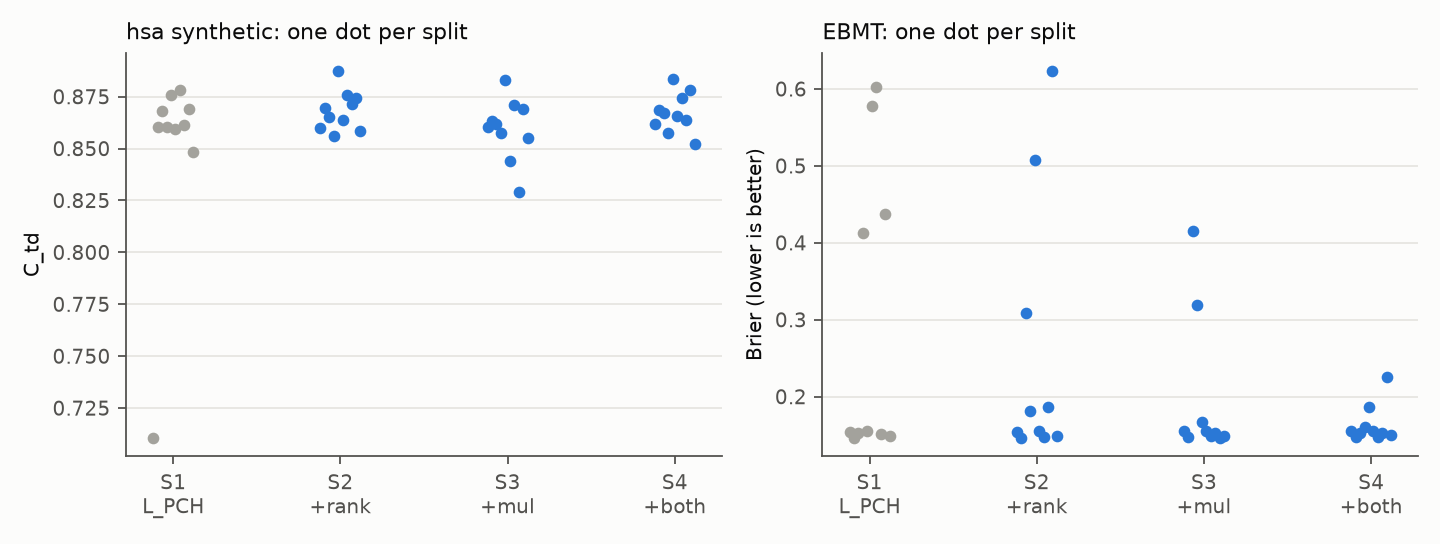
\includegraphics[width=0.8\textwidth]{losses_stability.png}
\caption{Every split of each loss variant. Left: $C_{td}$ on hsa synthetic. Right: Brier score on EBMT.
With $L_{PCH}$ alone (S1) some splits fail; with $L_{rank}+L_{mul}$ (S4) none do.}
\end{figure}

\section{Findings}
\begin{enumerate}
  \item \textbf{Our model is competitive but not the best.} It is in the upper half on every
        dataset and ties SurvTRACE on hsa synthetic, but wins no dataset. Our best variant is
        0.000--0.018 $C_{td}$ behind the best model.
  \item \textbf{$L_{rank}$ helps a little on every dataset} (S2 $\geq$ S1). The gain is
        statistically significant only on hsa synthetic.
  \item \textbf{The extra losses make training reliable.} With $L_{PCH}$ alone one hsa split
        collapses and several EBMT splits are badly calibrated. With $L_{rank}+L_{mul}$ (S4) this
        does not happen: the EBMT IBS drops from 0.338 to 0.233.
  \item \textbf{Adding the regression head does not hurt survival prediction} when $L_{rank}$ is
        used (``Full'' $\approx$ S2/S4).
  \item \textbf{Calibration is good} on four of five datasets, and better than SurvTRACE on
        METABRIC. EBMT is the exception.
  \item \textbf{EBMT is hard for every model} ($C_{td}$ 0.50--0.55): it has only four categorical
        features.
\end{enumerate}

\section{Conclusion}
The ranking losses of the paper do not make the model more accurate than the strongest baselines,
but they make it more reliable and better calibrated, and they allow the regression head to be
trained together with the survival head at no cost. The results do not support a claim of better
$C_{td}$ than SurvTRACE.

\end{document}
